%!TEX root = root.tex

\chapter{Statistically modeling the accumulation of somatic mutations in cancer}
\label{chap:ch2}
\chaptermark{Statistically modeling mutations}

Somatic mutations accumulate randomly in all cells of the body, starting from the beginning of embryogenesis through the entire lifetime of a person \cite{RN63}. Somatic mutations arise because of both endogenous and exogenous sources, or from a mutator phenotype acquired in a cancer cell. Endogenous sources include intrinsic DNA replication mistakes, damage caused by free radicals from metabolism, and spontaneous deamination of nucleotides \cite{RN64}. In contrast, exogenous sources originate from the environment and include ultraviolet radiation \cite{RN64} and various mutagenic chemicals like aristolochic acid \cite{RN65}.  Also, defective DNA damage repair in a cancer cell may lead to a mutator phenotype where a substantial number of unrepaired mutations become fixed, such as defective mismatch repair genes leading to microsatellite instability \cite{RN68}. Each mutational source leaves a mark on the cancer genome that reflects the mutational signatures during the lifetime of the cell's progeny leading to cancer \cite{RN64}.

\section{Variability in the background accumulation of mutations}

To investigate the potential for using elevated mutation rate per base as a means to detect cancer drivers, I sought to examine the background variability of mutation rate in human cancers. The median background mutation rate per base for each cancer type in my pan-cancer data set \cite{RN70} varied by over two orders of magnitude (\autoref{fig:mut_rate_variability}), with individual samples varying over an even larger range, which is consistent with prior observations \cite{RN13, RN51}. Because only a small fraction of the total somatic mutations in any common solid tumor affects driver genes, the remaining mutations can be considered passengers. The total number of mutations (drivers plus passengers) per base is therefore only slightly larger than the number of passenger mutations per base, and, for simplicity, I refer to this number as the background mutation rate. Mutation rates are also known to vary across the genome \cite{RN13} and are influenced by nucleotide context, gene expression, chromatin state, transcription factor occupancy, replication timing, DNA strand, and perhaps by a variety of factors that have yet to be discovered \cite{RN72, RN73, RN51, RN74}. For example, melanoma mutations in The Cancer Genom Atlas (TCGA) are predominately C to T transition mutations, which is not seen in other cancer types (\autoref{fig:mutation_context}).

\begin{figure}
  \centering
  \makeatletter
  \let\@currsize\normalsize
  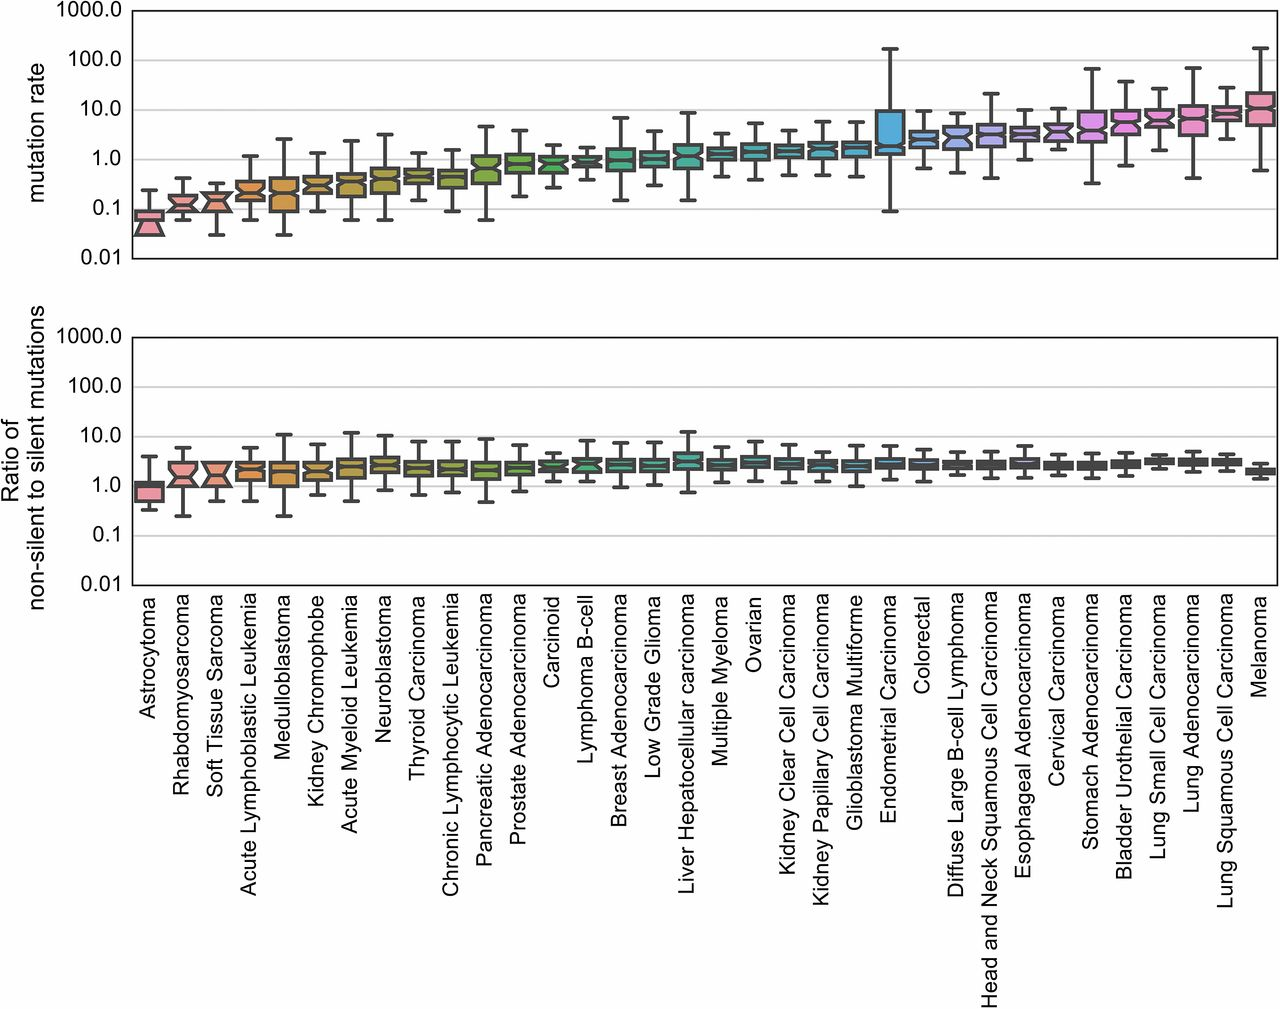
\includegraphics[width=0.9\linewidth]{figures/chapter2/mut_rate_and_ratiometric.jpg}
  \caption[Background mutation rate variability]{Background mutation rate is more variable than the ratio of nonsilent to silent mutations across 34 cancer types in data from \cite{RN14, RN71}. Boxplots are plotted on a log10 scale. The top boxplot shows the mutation rate in coding sequence for the samples in our pancancer dataset. The bottom boxplot shows the ratio of nonsilent to silent mutations in coding sequence for the same samples. A pseudocount for a silent mutation was added for each sample to avoid dividing by zero. Notches indicate bootstrap 95\% confidence interval (1,000 iterations) for the median. Outliers, defined as 1.5*IQR away from the first and third quartile, are not shown.}
  \label{fig:mut_rate_variability}
\end{figure}

\begin{figure}
  \centering
  \makeatletter
  \let\@currsize\normalsize
  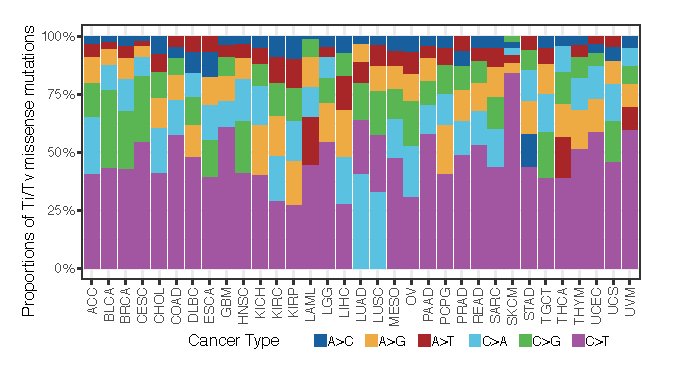
\includegraphics[width=0.9\linewidth]{figures/chapter2/mutation_context.pdf}
  \caption[Transition and transversion proportions in cancer]{Transition and transversion proportions are shown for 6 nucleotide changes from 33 cancer types available from the The Cancer Genome Atlas (https://synapse.org/MC3). The stacked proportion bar chart is sorted by increasing transition/transversion fraction.}
  \label{fig:mutation_context}
\end{figure}

However, mutation rate is not the only statistic capable of associating cancer drivers. One alternative is to use ratiometric features that normalize for the total number of mutations within a gene. For example, the ratio of non-silent to silent mutations within a gene is relative to silent mutations. \autoref{fig:mut_rate_variability} shows the variability of the median ratio of non-silent to silent mutations for cancer types in our pancancer set. Ratiometric features had significantly less variability among cancer types than background mutation rates. The considerably lower variability suggests less factors would need to be modeled when developing a statistical model of somatic mutations.

\section{Expected consequence of variable background mutation rate}

\subsection{Increased mutational heterogeneity results in reduced statistical power or increased false positives}

I analyzed the possible impact of unexplained variability in background mutation rate on expected false-positive driver gene predictions. First, I applied a binomial model previously used for driver gene detection power analysis \cite{RN14}. The model assumes a gene-specific background mutation rate $\mu$, which is set to a relatively high value, corresponding to genes in the 90th percentile of genes for mutation rate. I used the binomial to set a critical value for driver gene prediction, that is, the number of mutations required for a gene to be considered significantly different from the background. Next, I modeled the situation where the genes actually had mutation rates that varied around μ, using a beta-binomial model. I estimated the false positives expected under the binomial, after a highly conservative multiple-testing correction (Bonferroni), for levels of variability [beta-binomial coefficients of variation (CVs)], and for sample size ranging up to 8,000 (\autoref{fig:expected_fp}). Levels of variability defined by CVs (CV = 0.05, 0.1, and 0.2) were chosen to approximate low, medium, and high unexplained variation around the mean. As the number of samples increased, so did the number of expected false positives. At the low end of background mutation rates (0.5 mutations per megabase (MB)), the expected false positives remained low, even when 8,000 samples were evaluated, regardless of the level of variability. At an intermediate background mutation rate of 3.0 mutations per MB and with high unexplained variability, ∼1,000 false positives were expected from 8,000 samples. At a high background mutation rate (10.0 mutations per MB), both medium and high unexplained variability produced many thousand expected false positives.

\begin{figure}
  \centering
  \makeatletter
  \let\@currsize\normalsize
  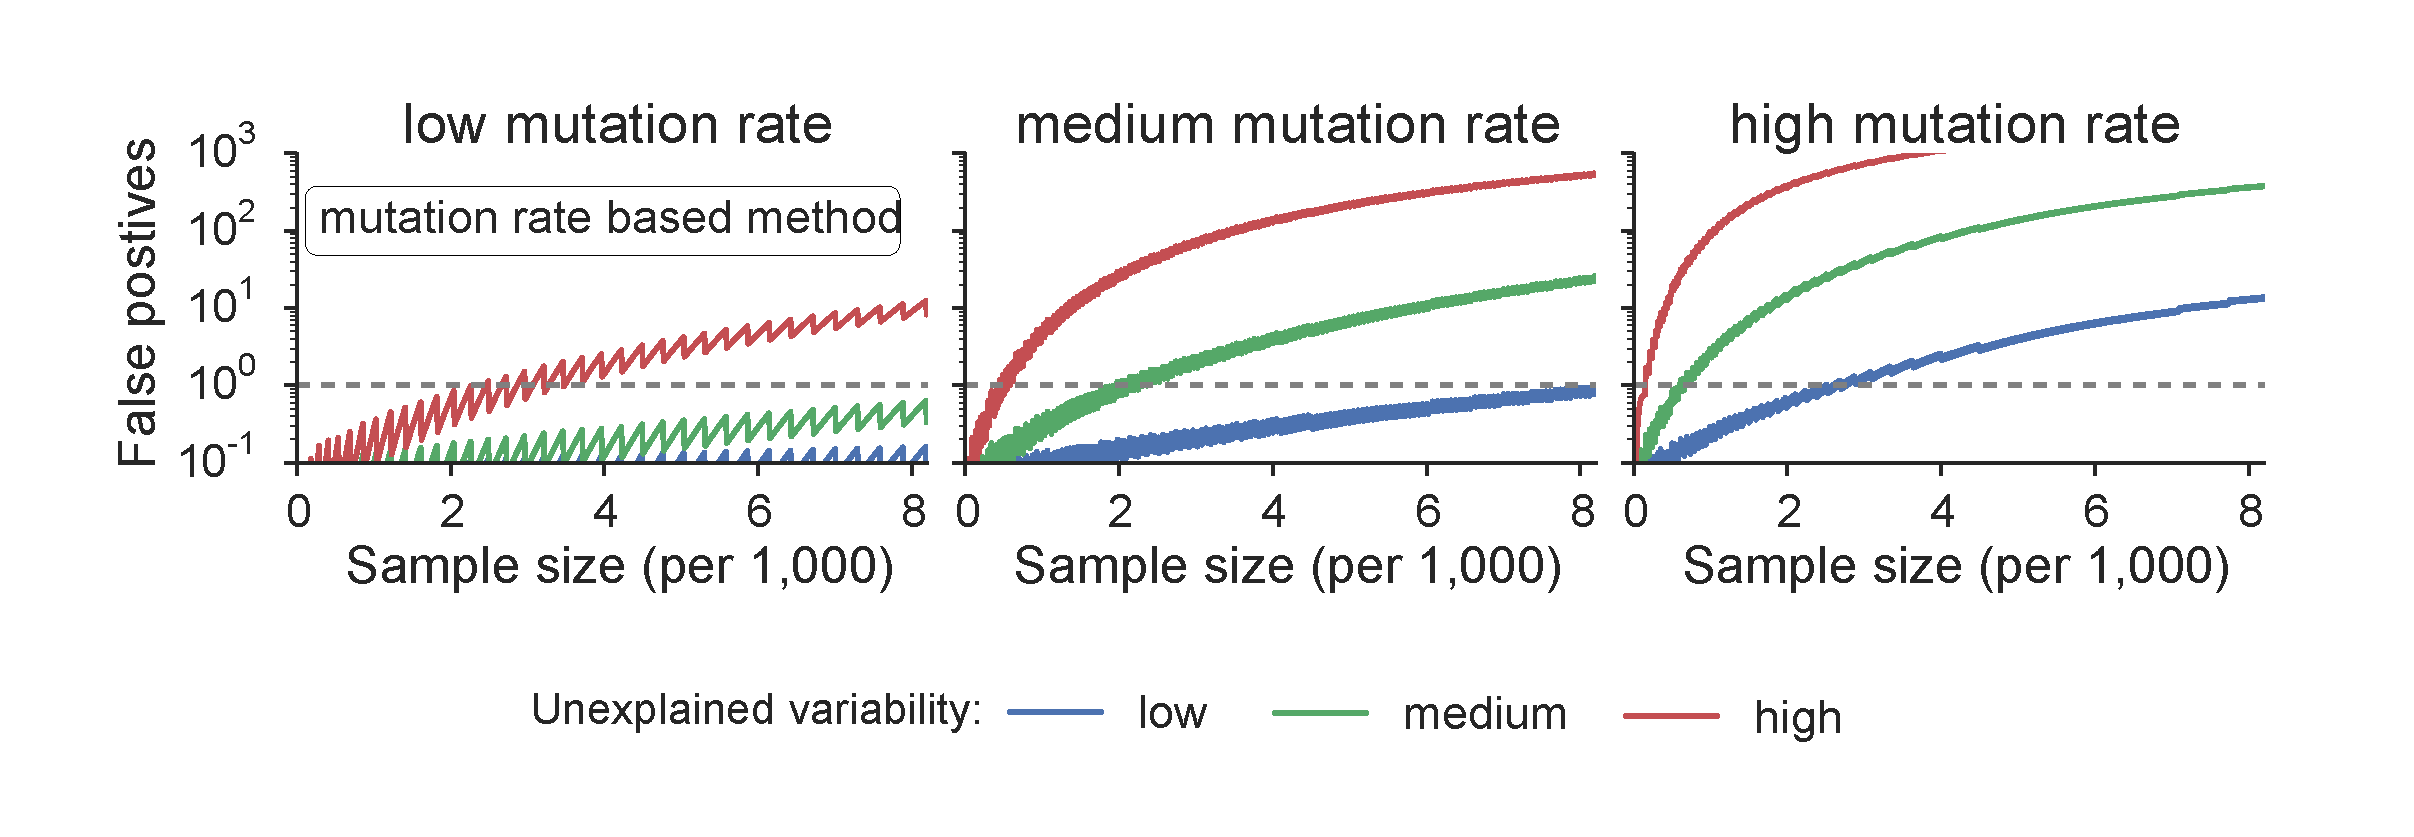
\includegraphics[width=0.9\linewidth]{figures/chapter2/expected_false_positives_mutation_rate.pdf}
  \caption[Expected false positives for driver gene detection]{Expected false positives for a mutation rate-based predictor that identifies genes with increased mutation rate over background.}
  \label{fig:expected_fp}
\end{figure}

I reasoned that unexplained variability might also have an impact on power calculations to estimate how many samples must be sequenced to find the majority of cancer driver genes. To this end, I repeated previous calculations performed with a binomial power model, in which the required sample size was estimated to be 600-5,000 per cancer type \cite{RN14}. The original model was parameterized to detect intermediate frequency driver genes, having 2-20\% mutation rates above background per sample, with background defined by genes in the 90th percentile of background mutation rates. First, I calculated the sample size required to detect 90\% of these drivers, given exome-wide backgrounds of 0.1-10 mutations per MB, and a conservative estimate of 2\% effect size (see statistical modeling of mutation rate). Next, I calculated the sample size required if the gene mutation rate varied around the original estimate, using a beta-binomial model with different CVs (CV = 0.05, 0.1, 0.2). The binomial power model was in accord with previous estimates. However, when unexplained variability was taken into account, the number of required samples increased sharply, particularly for higher background mutation rates (\autoref{fig:statistical_power}).

\begin{figure}
  \centering
  \makeatletter
  \let\@currsize\normalsize
  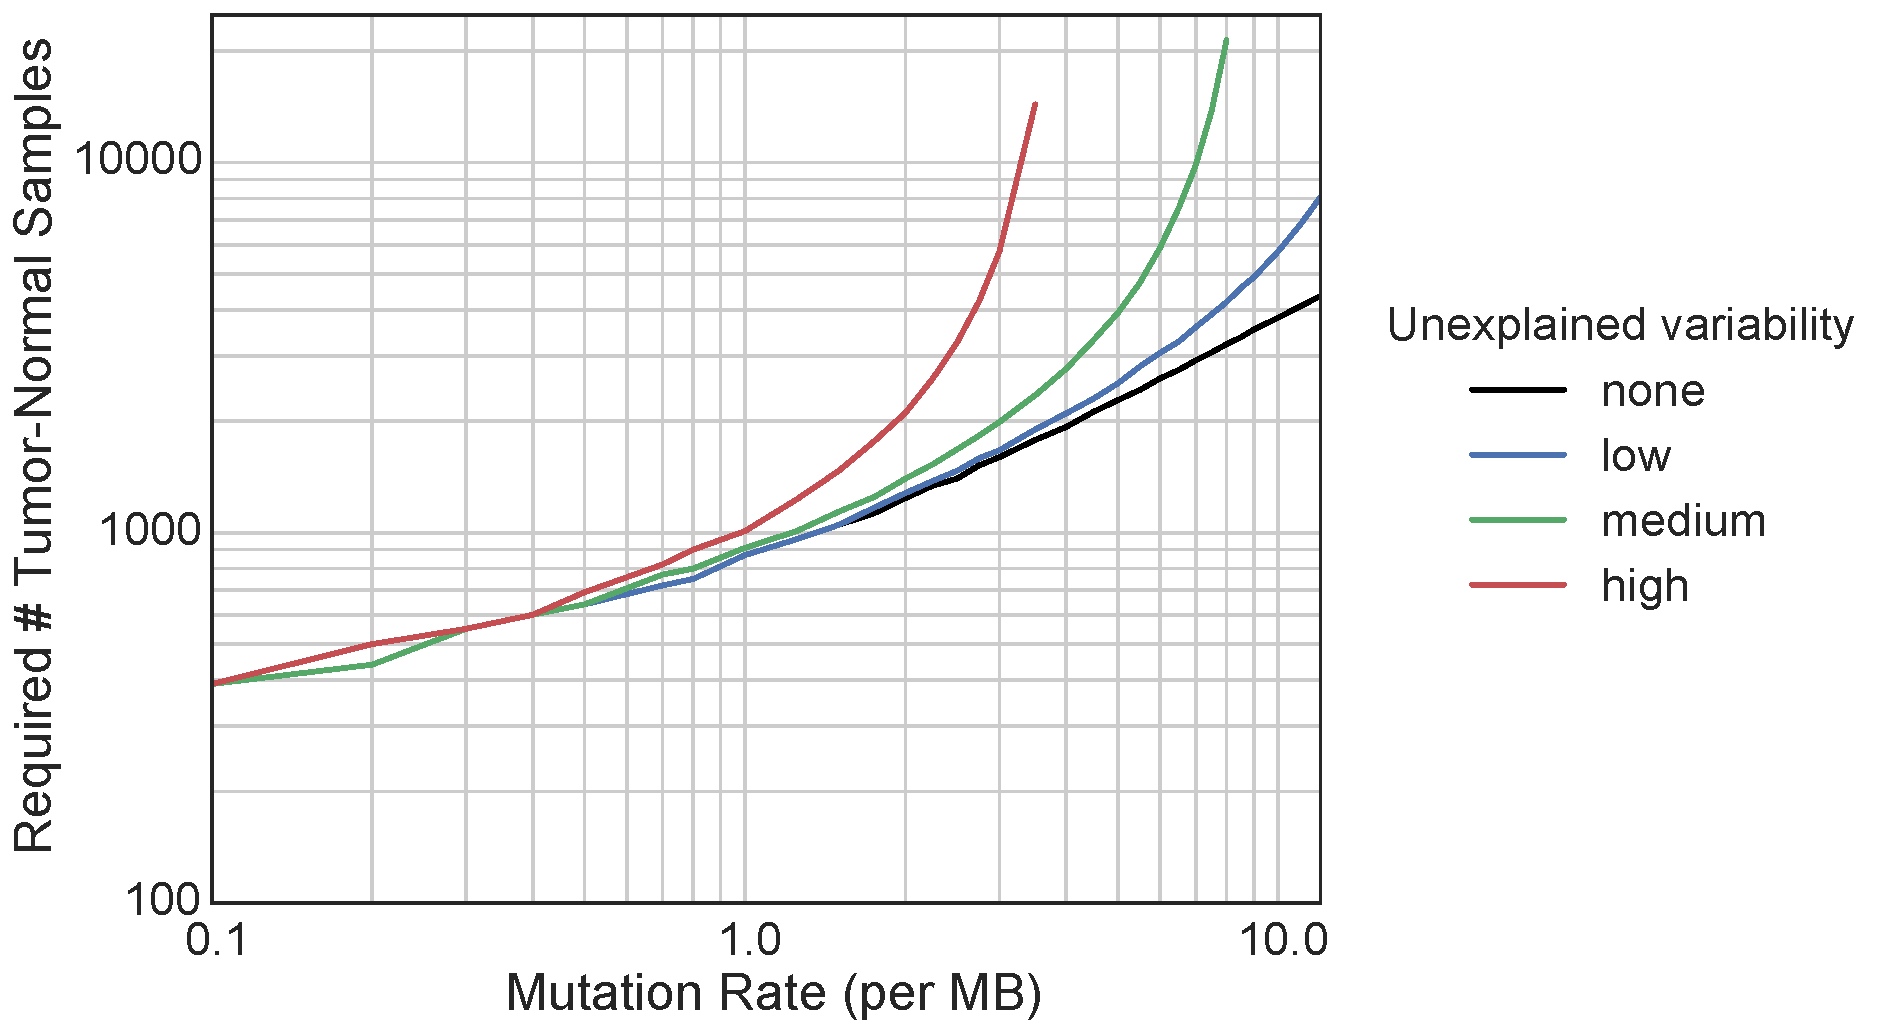
\includegraphics[width=0.9\linewidth]{figures/chapter2/statistical_power.pdf}
  \caption[Sample size required for near-comprehensive detection of driver genes]{Sample size required for near-comprehensive detection of intermediate-effect driver genes (90\% detection and 2\% effect size/increase with respect to background). Results are shown for scenarios with no unexplained variability (black), low (blue), medium (green), and high (red) unexplained variability (CVs of 0.0, 0.05, 0.1, and 0.2, respectively). The number of required samples for the mutation rate-based method becomes very large for moderate-to-high mutation rates and levels of unexplained variability.}
  \label{fig:statistical_power}
\end{figure}

\subsection{Statistical models of mutation rate}

Now I will describe the implementation of the statistical models used to evaluate the effects of unexplained variability in the mutation rate on false positives and statistical power. The first model assumes a correctly estimated background mutation rate μ for a particular gene (binomial model) and the second model assumes that gene background mutation rate varies around μ (beta-binomial model). I used a binomial model similar to previously developed for driver gene power analysis \cite{RN14}. The gene-specific mutation rate factor $F_g$ calculated by MutsigCV \cite{RN14} was set to represent a gene at the 90th percentile, given an exome-wide background mutation rate of $\pi$, so that $\mu=F_g\pi$ ($F_g$ = 3.9). Average gene length ($L$) was set to 1,500 bases and 3/4 mutations were assumed to be non-silent. Effective gene length for non-silent mutations was therefore adjusted as $L_{eff}=3/4L$. Gene background mutation rate was calculated using the total number of potentially mutated bases that could yield a non-silent mutation ($N_{eff}$), which is the effective gene length multiplied by number of samples ($S$). A predicted driver was defined as a gene with significantly higher non-silent mutation rate per base than that gene's background mutation rate, where non-silent mutation rate per base is the following:

\begin{equation}
\mu^{es} = 1 - ((1-\mu)^{L_{eff}}-r)^{1/L_{eff}}
\end{equation}

and $r$ is the fraction of samples with non-silent mutations in the gene above background. Exome-wide background mutation rates of ($\pi$ = 0.5e-6, 3e-6, or 10e-6) were considered.

The beta-binomial was designed to model several levels of unexplained variability around μ. To parameterize the beta-binomial with low, medium, and high variability levels, I used different coefficients of variation (CVs) for the mutation rate (0.05, 0.1, 0.2). Beta-binomial $\alpha$ and $\beta$ parameters were computed as follows:

\begin{equation}
\label{eq:alpha}
\alpha = \mu\left(\frac{\mu(1-\mu)}{(CV*\mu)^2}-1\right)
\end{equation}
\begin{equation}
\label{eq:beta}
\beta = (1-\mu)\left(\frac{\mu(1-\mu)}{(CV*\mu)^2}-1\right)
\end{equation}

To compute the number of false positives expected from a binomial model when unexplained variability is present, I examined the probability that the number of mutations in a gene from a beta-binomial model ($K_{bb}$) would meet or exceed the critical value (for a genome-wide significant driver gene at $\alpha$ = 5e-6) by the binomial, $k'_b$:

\begin{equation}
E[FP] = g*P_{\mu,N_{eff}}[K_{bb}\geq k'_b]
\end{equation}

where $g$ is the total number of human genes (assumed 18,500) and both models use the same mean mutation rate $\mu$ and total number of potentially mutated bases $N_{eff}$.

A similar model is applicable to the effect of various levels of unexplained variability in mutation rate on the power to detect driver genes. I reproduced the binomial model power analysis of \cite{RN14} to estimate the number of samples required for 90\% power to detect genes in the 90th percentile of gene-specific background rate, with 2\% mutation rate above background ($r$ = 0.02). Using Equations \ref{eq:alpha} and \ref{eq:beta} to parameterize the beta-binomial model, I calculated the number of samples required for 90\% power at a Bonferroni genome-wide significance level of 5e-6. Samples were iteratively added until there was greater than or equal to 90\% probability that a driver gene with mutation rate $\mu^{es}$ would be found significant. Because of the jagged power curve for discrete data \cite{RN75}, I found the minimum number of samples required to achieve 90\% power.

\section{A Monte Carlo simulation approach}
\label{sec:monte_carlo}

\subsection{Implementation}

Given the previously highlighted limitations of using the mutation rate, I decided to instead model ratiometric features and statistically condition on the total number of mutations within a gene. This strategy tries to limit the effect of nuisance factors influencing mutation rate that are not always measured or known. Briefly, for each gene, single nucleotide somatic mutations were moved with uniform probability to any matching position in the gene sequence, holding the total number of single nucleotide somatic mutations fixed (Fig. 5). A matching position was required to have the same nucleotide base context (C*pG, CpG*, TpC*, G*pA, A, C, G, T) as the observed position. This method of generating a null distribution controls for the particular gene sequence, gene length, and mutation base context. The number of somatic mutations remains the same, but the mutation consequence of a somatic mutation may change. For example, a somatic mutation that generates a missense mutation may generate a nonsense mutation in its new position. Since mutations that result in insertions and deletions will not change their mutation consequence type by being randomly moved to another position in the same gene, they were moved to a random position in a different gene. This gene was selected based on a multinomial model, with probability proportional to the coding DNA sequence length of the originating gene.

The simulated mutations allow calculating the statistical significance of an arbitrary test statistic computed from the mutation data. Let's say there is a function $T$ of some set of mutation(s) $M$. I can then compute an estimated p-value based on the simulated mutations $M^0$ as follows,

\begin{equation}
\widehat{P(M)} = \frac{\#\{T(M^0_i) : T(M^0_i) \geq T(M), i \in 1..S\}}{\#\{T(M^0_i) : i \in 1..S\}}
\end{equation}

where $\widehat{P(M)}$ is the estimated p-value and $S$ is the total number of simulations. 

\subsection{Comparison to simulations in CHASM}

There are several notable differences between my implemented Monte Carlo simulation procedure and that previously employed by the method Cancer-specific High-throughput Annotation of Somatic Mutations (CHASM) \cite{RN29}. First, mutations are simulated in a cohort-level manner, rather than considering each unique mutation in isolation. This allows computation of test statistics that may be a function of many mutations found in a single region, a single gene, or in multiple genes. Second, the original CHASM simulations assumed a background rate for mutations at certain nucleotide contexts (termed 'passenger tables'). Instead, I condition on the observed nucleotide context and randomly select another position with the same context. Third, I do not assume a homogenous mutation rate for single nucleotide mutations in genes across the genome. Fourth, my Monte Carlo simulations also apply to all coding mutations, rather than just missense mutations. Lastly, because driver genes may also contain passenger mutations, I do not blacklist simulated mutations in driver genes.

\subsection{Application to salivary gland adenoid cystic carcinoma (ACC)}

\subsubsection{ACC overview}

As part of the statistical analysis, I analyzed coding mutations from 25 whole-genome sequenced Adenoid Cystic Carcinomas (ACC) \cite{RN76}. Specifically, it was noticed that several chromatin regulator genes had more than one non-silent mutation. The question was whether these chromatin regulator genes had a high proportion of truncating mutations, suggesting that they could be tumor suppressor genes.

\subsubsection{Model of truncating point mutations}

I performed a randomization-based statistical test of increased proportion of truncating mutations ($K$) out of total non-silent mutations ($N$) for genes involved in chromatin regulation, controlling for the effect of gene sequence and mutational context. For each gene $i$, our test statistic was

\begin{equation}
T_i = \frac{\#\{t : t\in K\}}{|N|}, where K\subset N
\end{equation}

Truncating mutations were defined as any nonsense, conserved di-nucleotide splice-site mutations, or out-of-frame insertions/deletions (frameshift). Monte Carlo simulations were performed to approximate the null probability distribution of the test statistic $T_i$. Because frameshift mutations do not change consequence when moved to a different position, in the Monte Carlo sample, they were retained with probability equal to the observed proportion of frameshift mutations out of all mutations (maximum likelihood estimate), otherwise they were changed to a non-truncating mutation. After each iteration of this sampling procedure, the number of mutations in a gene is always the same, but the mutation consequence of each mutation may change. Thus, the test statistic $T_i$ for the gene will change values at each iteration, and repeated iterations yield a null distribution of test statistics to estimate the P value of the gene's observed test statistic. For the gene group analysis, my test statistic was

\begin{equation}
T_c = \frac{\sum_{i\in c}{\#\{t:t\in K_i\}}}{\sum_{i\in c}{|N_i|}}
\end{equation}

and it was computed both for the observed and simulated mutations. A one-tailed empirical P value was calculated as the fraction of Monte Carlo samples in which the observed value of the test statistic was equal to or higher than the simulated value. Increasing the number of iterations of Monte Carlo sampling increases the precision of the P value; 10,000,000 iterations were
chosen to achieve adequate precision.

\subsubsection{Results}

Several genes with well-known roles in chromatin regulation were mutated in multiple tumors: MLL2, MLL3, EP300, SMARCA2, SMARCC1, and KDM6A. The proportion of truncating mutations (nonsense codons, splice-site alterations, or out of-frame insertions and deletions) out of the total number of non-silent mutations in these genes was high (6 of 11), significantly greater than expected by chance (P = 3.8e-6). Furthermore, MLL2 and EP300, when considered individually, had a significantly higher proportion of truncating mutations than expected by chance (P = 0.008 for MLL2 and P = 0.01 for EP300). This finding is consistent with the hypothesis that several of these genes played an important role in the cancers in which they occurred.

\section{Conclusions}

The goal in this chapter was to first understand \q{how} somatic mutations accumulate in the absence of selection so as to, later, correctly interpret \q{which} mutations are cancer drivers in the presence of positive selection. A recent study indicates there is limited purifying selection of point mutations in cancer \cite{RN56}, suggesting the lack of incorporating negative selection in statistical models is not a major concern. I have shown in this chapter that background mutation rate is highly variable at multiple scales and therefore is difficult to statistically model. This can either lead to increased false positives or reduced statistical power when attempting to identify cancer driver genes. However, many of the known covariates modulate mutation rate at the scale of megabases within the genome \cite{RN74}, but nearly all genes span $<$1MB. I therefore developed Monte Carlo simulations to test any arbitrary test statistic by conditioning on the total number of mutations within a gene while accounting for nucleotide sequence context. The flexibility of the Monte Carlo simulations will be critical in later chapters when evaluating the significance of results from machine learning methods. 